\documentclass[a4paper,12pt]{article}
\usepackage{german}
\usepackage{times}
\usepackage{amsmath}
\usepackage{amssymb}
\usepackage{amsfonts}
\usepackage{amsthm}
\usepackage{graphicx}
\usepackage{textcomp}
\usepackage{txfonts}
\usepackage{geometry}
\geometry{papersize={210mm,297mm},total={160mm,240mm},top=31mm,bindingoffset=15mm}
\begin{document}
\title{"Aquivlentwiderstand von Kubooktaeder und Rhombendodekaeder}
\author{Andreas M"uller}
\date{}
\maketitle
\section{Einleitung}
Die Kirchhoffschen Regeln erlauben, die Str"ome zu berechnen,
die in einem beliebige Netzwerk von Widerst"anden und Spannungsquellen fliessen.
Die lineare Algebra stellt eine Reihe von Hilfsmitteln bereit, die
die Berechnung zu vereinfachen helfen.
Damit wird es m"oglich, auch exotische Netzwerke zu berechnen, zum Beispiel
solche, die als Kanten eines Polyeders auftreten.

Besonders interessant sind nat"urlich die platonischen K"orper Tetraeder, W"urfel,
Oktaeder, Dodekaeder und Ikosaeder, zu denen es in der Aufgabensammlung
einige Information gibt.
Insbesondere sind dort die "Aquivalentwiderst"ande eines mit
1k$\Omega$-Widerst"anden realisierten Kantennetzwerkes f"ur jeden 
platonischen K"orper berechnet worden.

Man stellt dabei auch interessante Zusammenh"ange zwischen sogenannt dualen
K"orpern fest.
Zwei K"orper heissen dual, wenn das Netzwerk der Kanten des einen aus dem des anderen
dadurch hervorgeht, dass man f"ur jede Seitenfl"ache einen Knoten bildet
und genau diejenigen Knoten miteinander "uber eine Kante verbindet, die zu
Seitenfl"achen geh"oren, die an einer Kante zusammenstossen.
Die Dualit"atsbeziehungen f"ur die platonischen K"orper sind:
\begin{center}
\begin{tabular}{ll}
\hline
K"orper&dazu dual\\
\hline
Tetraeder&Tetraeder\\
Hexaeder (W"urfel)&Oktaeder\\
Dodekaeder&Ikosaeder\\
\hline
\end{tabular}
\end{center}

\begin{figure}
\centering
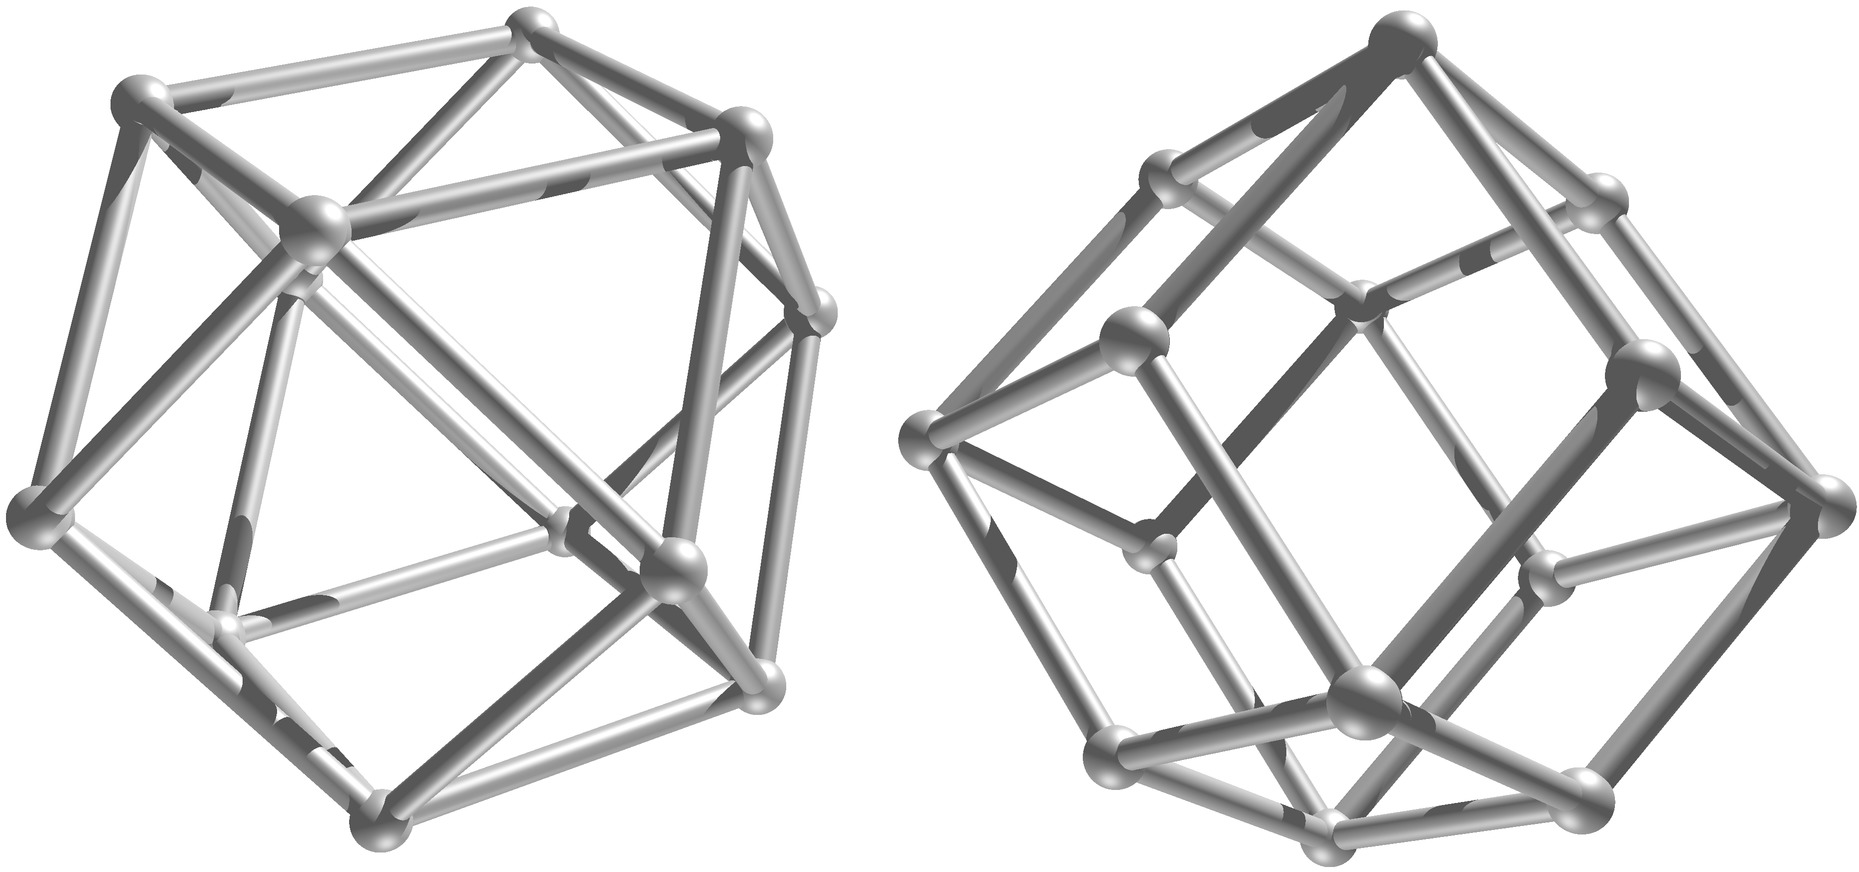
\includegraphics[width=\hsize]{kubooktaeder.jpg}
\caption{Kantennetzwerk von Kubooktaeder (links) und Rhombendodekaeder (rechts)
\label{kantennetzwerke}}
\end{figure}
\begin{figure}
\centering
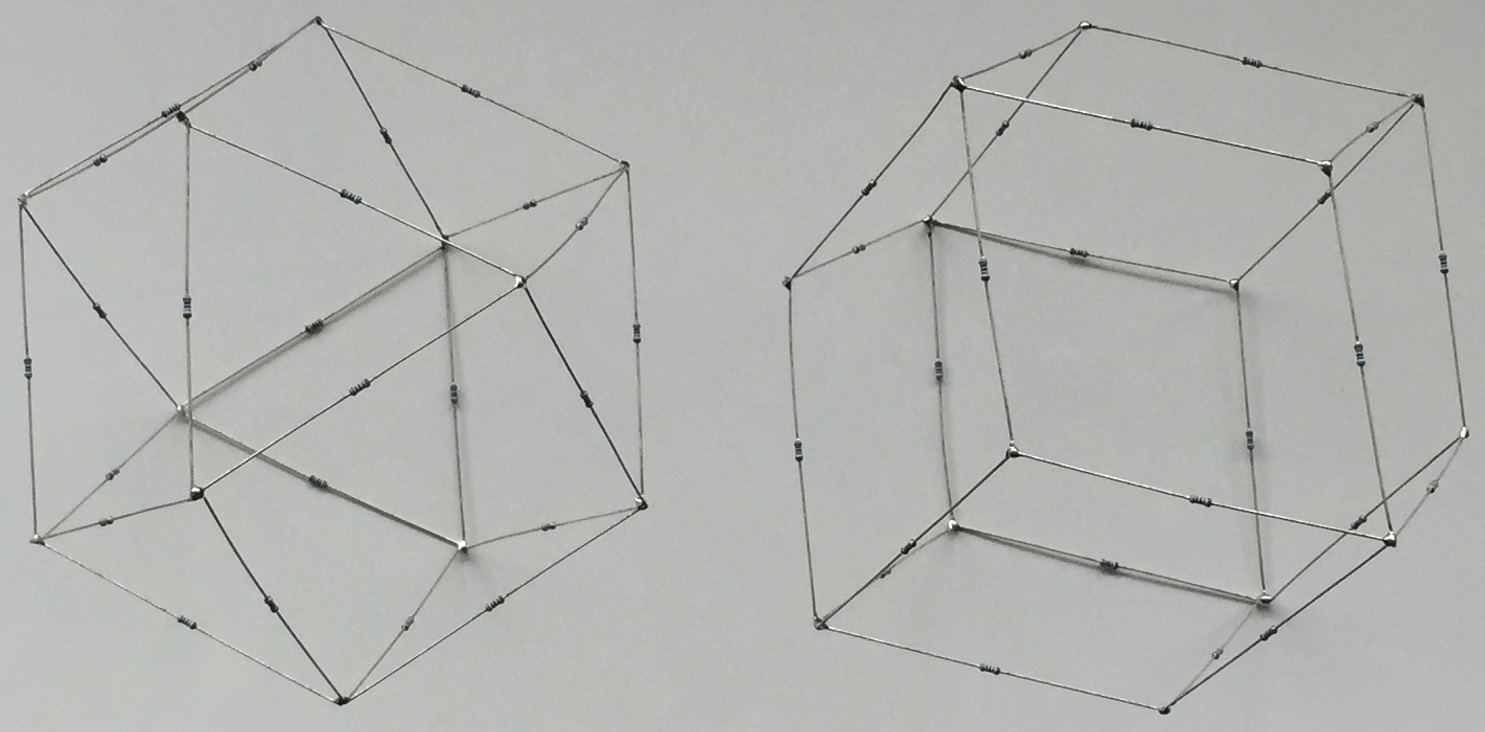
\includegraphics[width=\hsize]{realization.jpg}
\caption{Realisierung des Kantennetzwerks von Kuboktaeder (links)
und Rhombendodekaeder (rechts) mit 1k$\Omega$-Widerst"anden.
\label{realization}}
\end{figure}
Schneidet man einem W"urfel die Ecken durch Ebenen ab, die durch die Kantenmitten
gehen, erh"alt man ein neues Polyeder aus sechs Quadraten und acht gleichseitigen
Dreiecken, ein sogenanntes Kubooktaeder (Abbildung~\ref{kantennetzwerke}, links).
Es besteht aus acht gleichseitigen Dreiecken und sechs Quadraten.
Den gleichen K"orper k"onnte man auch erhalten, indem man einem Oktaeder
die Ecken durch Ebenen durch die Kantenmitten abschneidet,
was den Namen plausibel macht.
Der dazu duale K"orper ist das Rhombendodekaeder, es besteht aus zw"olf Rhomben.

Die Dualit"at von Kubooktaeder und Rhombendodekaeder spiegelt sich auch in
den Symmetrieeigenschaften der Ecken und Seitenfl"achen.
Beim Kubooktader treffen in allen Ecken vier Kanten zusammen, aber in
verschiedenen Winkeln ($60^\circ$ und $90^\circ$).
Beim Kubooktaeder gibt es also nur eine Art von Ecken, aber zwei Arten von
Seitenfl"achen.
Beim Rhombendodekaeder dagegen gibt es nur eine Art von Seitenfl"achen,
aber zwei verschiedene Arten von Ecken, in denen drei oder vier
Kanten zusammentreffen.
Sie entsprechen nat"urlich den zwei verschiedenen Seitenfl"achen des 
Kubooktaeders.

Man kann das Rhombendodekaeder "ubrigens nicht dadurch erhalten, dass man
einfach die Seitenmitten des Kubooktaeders miteeinander verbindet, denn die
Mitten der quadratischen Seitenfl"achen des Kubooktaeders liegen in der
gleichen Ebene wie zwei der Kanten der Dreiecksfl"achen.
Dies kann man auch in Abbildung~\ref{kantennetzwerke} sehr sch"on sehen.

Umgekehrt ist das Kubooktaeder tats"achlich dadurch realisierbar, dass
man die Seitenmitten des Rhombendodekaeders verbindet, was zum Beispiel
daraus folgt, dass man beim Rhombendodekaeder in jeder $n$-z"ahligen
Ecke (Ecke mit $n$ Kanten) auch eine $n$-fache Rotationssymmetrie hat,
w"ahrend beim Kubooktaeder in den 4-z"ahligen Ecken zwei Quadrate
und zwei Dreiecke zusammenkommen, so dass dort nur eine
$180^\circ$-Rotationssymmetrie m"oglich ist.

\section{Aufgabenstellung}

\newtheorem{aufgabe}{Aufgabe}
\begin{aufgabe}
Man berechne die "Aquivalentwiderst"ande "uber eine Kante eines mit
1k$\Omega$-Widerst"anden realisierten Kubookateders und eines Rhombendodekaeders.
\end{aufgabe}

{\parindent0pt \bf Wettbewerbsbedingungen:}
\begin{enumerate}
\item
Die L"osung muss so dokumentiert sein, dass sie ohne weitere Hilfsmittel
nachvollziehbar ist.
\item
Es ist zul"assig, ein Computerprogramm zu verwenden, welches aber ebenfalls
soweit dokumentiert sein muss, dass man es nicht selbst kompilieren oder
ausf"uhren muss um zu verstehen, wie es funktioniert.
\item
Zur Kontrolle der eigenen L"osung stehen die Realisationen der beiden
Netzwerke zum Nachmessen zur Verf"ugung (Abbildung~\ref{realization}).
\item
Eingabefrist: 1.~November 2015, 00:00 Uhr.
\item
"Uber den Wettbewerb wird keine Korrespondenz gef"uhrt.
\end{enumerate}

\section{L"osung}
\dots
\end{document}
